
\section{Phân tích và Thiết kế hệ thống}

\subsection{Phân tích yêu cầu hệ thống (Requirement Analysis)}
Dựa trên các thách thức của mô hình mạng truyền thống và nhu cầu bảo mật hiện đại, hệ thống cần đáp ứng các yêu cầu cốt lõi sau:

\begin{itemize}
\item \textbf{Yêu cầu về bảo mật (Security)}:
\begin{itemize}
\item Loại bỏ sự phụ thuộc vào tường lửa truyền thống và địa chỉ IP tĩnh.
\item Đảm bảo mọi request phải được xác thực danh tính (Authentication) và kiểm tra quyền hạn (Authorization) trước khi mã nguồn được thực thi.
\end{itemize}
\item \textbf{Yêu cầu về hạ tầng (Infrastructure)}:
\begin{itemize}
\item Giảm thiểu gánh nặng quản trị máy chủ (No-Ops).
\item Hệ thống phải có khả năng chống đỡ các cuộc tấn công từ chối dịch vụ (DDoS) ngay từ lớp biên mạng.
\end{itemize}
\item \textbf{Yêu cầu về trải nghiệm người dùng (Performance)}:
\begin{itemize}
\item Quá trình xác thực phải diễn ra nhanh chóng, giảm thiểu độ trễ (latency) khi điều hướng giữa IdP và ứng dụng.
\end{itemize}
\end{itemize}

\subsection{Thiết kế kiến trúc dựa trên nhu cầu (Design Driven by Needs)}
Để đáp ứng các yêu cầu trên, dự án lựa chọn mô hình \textbf{Serverless Zero Trust Edge}. Đây là sự kết hợp giữa triết lý Zero Trust và sức mạnh của điện toán biên.

Kiến trúc được chia thành ba lớp chức năng độc lập nhưng phối hợp chặt chẽ:

\begin{itemize}
\item \textbf{Lớp định danh (Identity Layer - Keycloak)}:
Đóng vai trò là "Cội nguồn sự thật" (Source of Truth). Đáp ứng nhu cầu quản lý tập trung tài khoản và phân nhóm người dùng. Sử dụng giao thức OIDC để cấp phát định danh dưới dạng các Claims bảo mật.

\item \textbf{Lớp thực thi chính sách (Policy Enforcement Layer - Cloudflare Access)}: 
Đóng vai trò là Identity-Aware Proxy (IAP). Đáp ứng nhu cầu "Xác thực trước, truy cập sau". Lớp này ngăn chặn mọi truy cập trái phép ngay tại trung tâm dữ liệu gần người dùng nhất của Cloudflare.

\item \textbf{Lớp tính toán biên (Edge Compute Layer - Cloudflare Workers)}: 
Đóng vai trò là nơi chứa mã nguồn ứng dụng. Đáp ứng nhu cầu loại bỏ hạ tầng vật lý. Worker nhận dữ liệu định danh đã được IAP xác thực thông qua Header để xử lý logic nghiệp vụ.
\end{itemize}


\subsection{Quy trình luồng dữ liệu (Data Flow Diagram)}
Luồng xử lý được thiết kế theo các bước tuần tự để đảm bảo tính toàn vẹn và bảo mật:

\begin{itemize}
    \item \textbf{1. Yêu cầu(Request)}: Người dùng truy cập URL ứng dụng (Worker URL).

    \item \textbf{2. Chặn \& Điều hướng}: Cloudflare Access kiểm tra Session. Nếu chưa có, hệ thống thực hiện Điều hướng sang Keycloak qua giao thức OIDC.

    \item \textbf{3. Xác thực(Authentication)}: Người dùng đăng nhập tại Keycloak. Keycloak phát hành ID Token chứa các Claims (như groups, roles, department).

    \item \textbf{4. Claim Mapping \& Policy}: Cloudflare nhận Token, bóc tách các Claims đã cấu hình và đối chiếu với nguyên tắc(Policy). Nếu thỏa mãn, yêu cầu được cho phép đi tiếp.

    \item \textbf{5. Worker Execution}: Sau khi vượt qua lớp bảo mật, Mã nguồn trên Worker xử lý các yêu cầu(request) từ người dùng.

    \item  \textbf{6. Identity Awareness}: Mã nguồn ứng dụng bên trong Worker đọc các Header định danh (như cf-access-claims-groups) để quyết định hiển thị nội dung gì cho người dùng.
\end{itemize}

\begin{figure}[H]
    \centering
    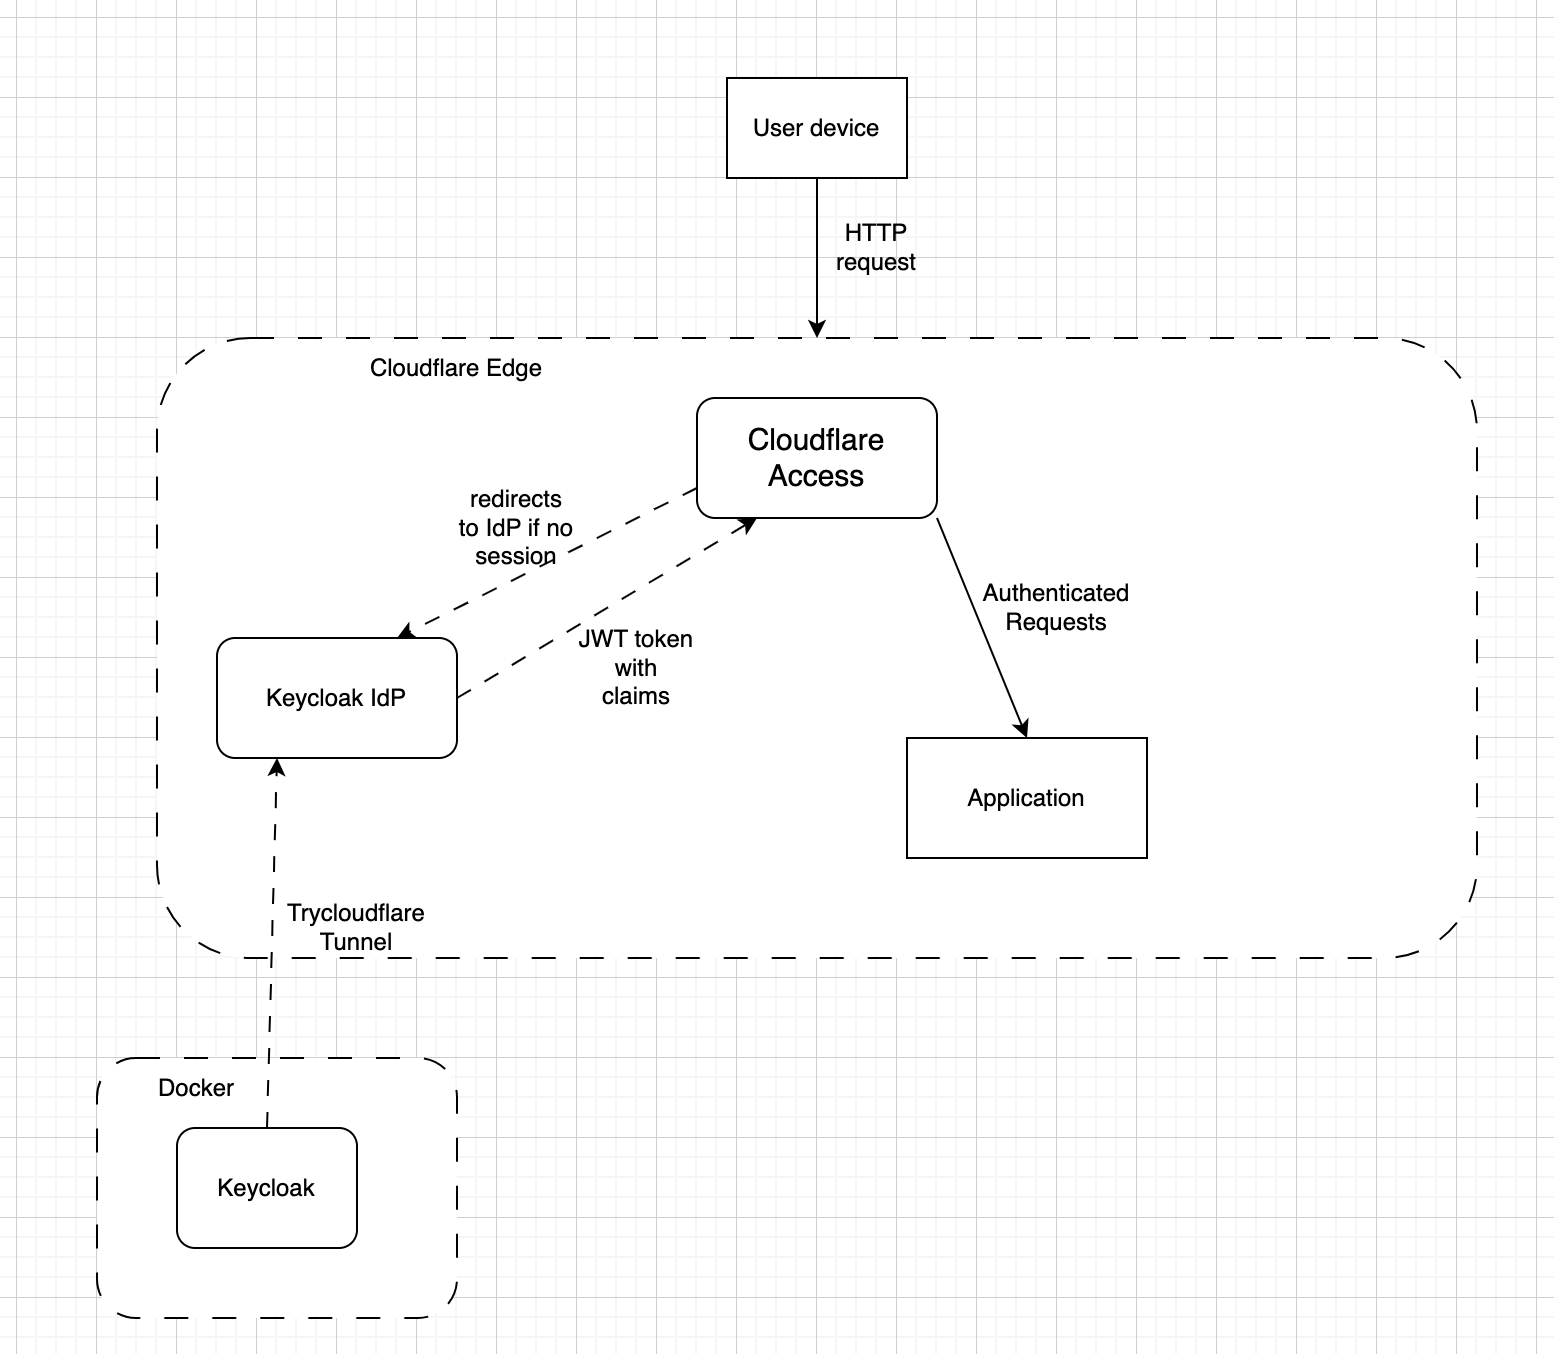
\includegraphics[width=0.5\textwidth]{contents/contents/image_11.png}
    \caption{Luồng thực thi của hệ thống}
    \label{fig:example_image}
    
\end{figure}

\subsection{Thiết kế kỹ thuật và đặc trưng}
Vì ứng dụng chạy ngay trên Worker, việc phân quyền không cần qua một "đường ống" nào mà được xử lý trực tiếp bằng code:

Đầu vào: Yêu cầu gồm các tiêu đề(headers) chứa các thông tin định danh đã được Cloudflare Access xác thực và lấy được thông qua claim dữ liệu từ keycloak.

Logic: Sử dụng mã JavaScript/TypeScript để kiểm tra quyền hạn (ví dụ: if (groups.includes('admin')) { ... }).

Zero Infrastructure: Không cần quản lý server, không cần lo về Tunnel hay mở port.

Tính sẵn sàng cao: Ứng dụng chạy trên hạ tầng toàn cầu của Cloudflare, tự động mở rộng theo lượng truy cập.

Bảo mật: Code chỉ chạy sau khi đã qua lớp lọc của Cloudflare Access. Nếu không có token hợp lệ, ngay cả yêu cầu cũng không đến được worker.

\subsection{Đánh giá giải pháp thiết kế}

Việc lựa chọn thiết kế này mang lại các giá trị thực tiễn vượt trội so với mô hình truyền thống:

\begin{table}[H]
\centering
\caption{Đánh giá giải pháp thiết kế dựa trên nhu cầu thực tế}
\label{tab:design_evaluation}
\renewcommand{\arraystretch}{1.5}
% Đảm bảo đã khai báo \usepackage[table]{xcolor} ở đầu file
\begin{tabular}{|p{3.5cm}|p{5cm}|p{5.5cm}|}
\hline
\textbf{Vấn đề đặt ra} & \textbf{Giải pháp thiết kế} & \textbf{Kết quả đạt được} \\ \hline
Nguy cơ lộ IP máy chủ & Chạy trực tiếp trên Workers & Không có máy chủ vật lý, không có IP để tấn công. \\ \hline
Độ trễ khi xác thực & Sử dụng QUIC Domain cho IdP & Tối ưu hóa tốc độ điều hướng và bắt tay TLS. \\ \hline
Phân quyền phức tạp & Phân quyền dựa trên tiêu đề claims từ danh tính người dùng & Phân quyền trực tiếp trong code dựa trên Claim từ Keycloak. \\ \hline
Chi phí hạ tầng & Serverless Model & Không tốn chi phí vận hành, bảo trì máy chủ 24/7. \\ \hline
\end{tabular}
\end{table}